\documentclass{rapportPfe}

\usepackage{url}
\usepackage[Lenny]{fncychap} % Ou try Lenny, Bjarne, Glenn, etc.
\usepackage{lipsum}
\usepackage{minted}
\definecolor{bg}{rgb}{0.95,0.95,0.95}

\usepackage{titlesec} % For customizing chapter and section titles
\usepackage{tocloft}  % For customizing the table of contents
\usepackage{hyperref} % For hyperlinks

\title{Système de gestion d'un laboratoire de recherche}

\begin{document}

%----------- Informations du rapport ---------

\titre{Système de gestion d'un laboratoire de recherche}
\sujet{Projet de Fin d'Année}

\enseignant{Professeur  \textsc{Khawla Asmi}}

\eleves{%
    El Araby \textsc{El Mahdi} \\
    Ossama \textsc{El Khalfi}
}

\jury{%
    Professeur \textsc{Soukaina Bouarourou}
}

%----------- Initialisation -------------------

\fairemarges
\fairepagedegarde

%-------------- Pages préliminaires --------------

\chapter*{Remerciements}
\addcontentsline{toc}{chapter}{Remerciements}
Nous remercions chaleureusement l’équipe pédagogique de l’Université Mohammed V pour son accompagnement durant ce projet. Nos remerciements s’adressent également à notre encadrant pour ses conseils avisés et à nos proches pour leur soutien.

\chapter*{Résumé}
\addcontentsline{toc}{chapter}{Résumé}
Ce rapport présente le développement d’un système centralisé destiné à la gestion d’un laboratoire de recherche, en réponse aux limites des méthodes traditionnelles. L’application permet d’automatiser les processus administratifs, de faciliter la communication entre chercheurs et de renforcer la sécurité des données. Ce travail s’inscrit dans le cadre du projet de fin d’année à l’Université Mohammed V.

\chapter*{Liste des Abréviations}
	\addcontentsline{toc}{chapter}{Liste des Abréviations}
	\begin{itemize}
	  \item \textbf{API} : Application Programming Interface
	  \item \textbf{UI} : User Interface
	  \item \textbf{DB} : Database
	  \item \textbf{CRUD} : Create, Read, Update, Delete
	  \item \textbf{ORM} : Object-Relational Mapping
	  \item \textbf{Rust} : Un langage de programmation système
	  \item \textbf{Node.js} : Un environnement d'exécution JavaScript côté serveur
	  \item \textbf{TypeScript} : Un superset typé de JavaScript
	  \item \textbf{WebSockets} : Une technologie de communication en temps réel
	  \item \textbf{Next.js} : Un framework React pour la création d'applications web
	  \item \textbf{PostgreSQL} : Un système de gestion de base de données relationnelle
	  \item \textbf{Prisma} : Un ORM pour les bases de données SQL
	  \item \textbf{Docker} : Un outil de conteneurisation
	  \item \textbf{Python} : Un langage de programmation
	  \item \textbf{FastAPI} : Un framework web modern et rapide pour Python
	  \item \textbf{NLP} : Natural Language Processing (Traitement du langage naturel)
	  \item \textbf{JWT} : JSON Web Token (jeton web JSON)
	  \item \textbf{RBAC} : Role-Based Access Control (contrôle d'accès basé sur les rôles)
	  \item \textbf{ACID} : Atomicité, Cohérence, Isolation, Durabilité (propriétés des transactions)
	  \item \textbf{SSR} : Server-Side Rendering (rendu côté serveur)
	  \item \textbf{SSG} : Static Site Generation (génération de site statique)
	  \item \textbf{DBeaver} : Un outil de gestion de base de données
	  \item \textbf{Kubernetes} : Un système d'orchestration de conteneurs
	  \item \textbf{GitHub} : Un service d'hébergement de répertoires Git en ligne
	  \item \textbf{CI/CD} : Intégration Continue / Déploiement Continu
	\end{itemize}

\newpage
\chapter*{Introduction générale}
\addcontentsline{toc}{chapter}{Introduction générale}

La gestion d’un laboratoire de recherche moderne représente un défi multidimensionnel, nécessitant une coordination rigoureuse des activités scientifiques, administratives et collaboratives. Les enjeux majeurs incluent l’optimisation des processus de publication, le suivi des participations aux conférences, la facilitation des échanges et la sécurisation des données de recherche.

Actuellement, de nombreux laboratoires recourent à des méthodes de gestion traditionnelles, reposant sur des outils bureautiques non spécialisés (tableurs, messageries électroniques, systèmes de stockage génériques). Bien que ces solutions soient largement répandues, elles présentent des lacunes significatives : redondance des tâches, dispersion des informations, risques d’erreurs et absence de centralisation. Ces limitations entravent la productivité scientifique et compliquent la prise de décision stratégique.

Dans ce contexte, le développement d’une application web dédiée à la gestion des laboratoires de recherche s’impose comme une solution incontournable. Une telle plateforme permettrait d’automatiser les processus répétitifs, de structurer la collaboration et d’assurer une meilleure traçabilité des données, tout en renforçant la sécurité et l’accessibilité de l’information.

\newpage
\tabledematieres

\newpage
\listoffigures

%------------ Corps du rapport ----------------

\chapter{Généralités sur le projet}

\section{Problématique}

La gestion efficace d’un laboratoire de recherche repose sur la coordination fluide des activités scientifiques, administratives et humaines. Pourtant, de nombreux laboratoires continuent d’utiliser des approches archaïques, souvent basées sur des outils génériques, peu adaptés à la complexité croissante de la recherche contemporaine. Cette situation engendre de nombreuses limites que nous analysons ci-dessous.

\subsection{Une Gestion Manuelle Fragmentée et Source d’Incohérences}

Les laboratoires s’appuient encore trop souvent sur des solutions non spécialisées comme les tableurs ou les échanges de courriels pour suivre les publications, projets, conférences et collaborations.

\begin{itemize}
  \item \textbf{Suivi imprécis et chronophage} : La saisie manuelle des données entraîne des erreurs fréquentes, une mise à jour fastidieuse et une perte de temps considérable, nuisant à la fiabilité du suivi scientifique.
  \item \textbf{Données dispersées et non structurées} : Les informations sont stockées dans des fichiers multiples et non synchronisés, rendant difficile l’obtention d’une vue d’ensemble cohérente et à jour.
  \item \textbf{Vulnérabilité accrue des données} : L’absence de protocoles robustes de sauvegarde et de sécurité expose les fichiers à des risques de perte, de corruption ou d’accès non autorisé.
\end{itemize}

\subsection{Communication Désorganisée et Collaboration Sous-Exploitées}

La réussite d’un laboratoire dépend de la qualité des échanges entre ses membres. Cependant, les outils de communication utilisés ne sont ni centralisés ni adaptés à un environnement scientifique.

\begin{itemize}
  \item \textbf{Canaux de communication éparpillés} : Entre messageries personnelles et échanges informels, la traçabilité et la conservation des discussions deviennent difficiles.
  \item \textbf{Faible intégration des outils collaboratifs} : L'absence de solutions intégrées et spécialisées freine la coordination et crée des silos informationnels.
\end{itemize}

\subsection{Défauts de Sécurité et Faible Capacité d'Évolution}

Les systèmes traditionnels, souvent construits de manière ad hoc, présentent des failles critiques.

\begin{itemize}
  \item \textbf{Contrôle d’accès rudimentaire} : La gestion des rôles et des permissions est inexistante ou limitée, ce qui compromet la confidentialité des données sensibles.
  \item \textbf{Infrastructure hétérogène et difficile à maintenir} : La coexistence d’outils isolés rend la maintenance complexe, coûteuse et sujette aux pannes.
  \item \textbf{Absence de scalabilité} : Ces systèmes ne sont pas conçus pour évoluer avec l’augmentation du nombre d’utilisateurs, de projets ou du volume de données, limitant leur durabilité.
\end{itemize}

\section{L’objectif à réaliser}

\subsection{Objectif Principal}
Développer une application web centralisée, sécurisée, performante et ergonomique pour optimiser la gestion des laboratoires de recherche. Elle repose sur une architecture à microservices, une base de données PostgreSQL, et un outil d’intelligence artificielle en Python pour résumer automatiquement les publications scientifiques.

\subsection{Fonctionnalités Principales}
\begin{itemize}
  \item \textbf{Suivi des publications et conférences} : Vision synthétique et historique complet, avec génération automatique de résumés via l’IA.
  \item \textbf{Messagerie instantanée} : Communication en temps réel entre les membres.
  \item \textbf{Gestion des droits d’accès} : Permissions avancées selon le rôle (administrateur, chercheur, responsable).
\end{itemize}

\subsection{Objectifs Secondaires}
\begin{itemize}
  \item Automatiser les tâches pour libérer du temps.
  \item Centraliser les échanges et favoriser la collaboration.
  \item Assurer la pérennité, la sécurité et la traçabilité des données.
  \item Créer une solution évolutive et maintenable sur le long terme.
\end{itemize}


\chapter{Spécification des besoins}

L’architecture backend de cette application repose sur une conception modulaire et distribuée, mettant l’accent sur la séparation claire des responsabilités. Cette méthode vise à maximiser la facilité de maintenance, la possibilité d’évolution indépendante des services, ainsi que la robustesse globale du système. Chaque service, dédié à une fonction métier spécifique, est développé avec la technologie la plus appropriée à ses besoins, tout en s’intégrant harmonieusement dans l’ensemble de l’écosystème applicatif.

\section{Service de gestion des publications et conférences : \texttt{Rust}}

Ce service est développé en Rust, en réponse à des exigences strictes de performance, fiabilité et sécurité. Il gère l’ensemble du cycle de vie des publications et conférences à travers des API performantes, incluant un service dédié au téléversement de fichiers ainsi qu’un point de terminaison pour l’observation de métriques internes.

\begin{itemize}
    \item \textbf{Performance et gestion efficace des ressources :} Rust compile en code natif performant, proche du C/C++, sans ramasse-miettes, ce qui est essentiel pour traiter de gros volumes de données bibliographiques et de fichiers.
    \item \textbf{Sécurité mémoire et fiabilité :} Le système d’emprunt de Rust élimine les erreurs mémoire à la compilation, garantissant l’intégrité des données même dans des scénarios à forte charge.
    \item \textbf{Service de téléversement :} Un composant dédié en Rust prend en charge le téléversement sécurisé des fichiers de publication (PDF, documents complémentaires), avec vérification, stockage et association automatique aux métadonnées.
    \item \textbf{Point de terminaison de métriques :} Le service expose un point de terminaison \texttt{/metrics} personnalisé, fournissant des statistiques internes telles que le nombre de téléversements, les temps de réponse, les erreurs rencontrées ou encore l’état des composants, facilitant la supervision et le diagnostic.
    \item \textbf{Gestion avancée de la concurrence :} Grâce au modèle de possession de Rust, le traitement simultané des requêtes est effectué de manière sûre, sans accès concurrent dangereux à la mémoire.
\end{itemize}

Rust s’avère donc particulièrement adapté aux systèmes critiques nécessitant robustesse, performance et observabilité. Il bénéficie également d’un écosystème web moderne (\texttt{Axum}, \texttt{SQLx}, etc.) facilitant la construction d’API web fiables et maintenables.

Rust est donc particulièrement adapté aux systèmes critiques. Il bénéficie par ailleurs d’un écosystème web moderne (\texttt{Axum}, \texttt{SQLx}, etc.) permettant la création d’API web performantes et robustes.

Rust est donc particulièrement adapté aux systèmes critiques. Il bénéficie par ailleurs d’un écosystème web moderne (\texttt{Axum}, \texttt{SQLx}, etc.) permettant la création d’API web performantes et robustes.

Rust est donc particulièrement adapté aux systèmes critiques et bénéficie d’un écosystème web solide pour des API robustes.

\section{Service d’authentification et gestion des identités : \texttt{Node.js} avec \texttt{TypeScript}}

Ce service gère l’authentification avec Node.js et TypeScript, pour combiner rapidité de développement et sécurité.

\begin{itemize}
    \item \textbf{Modèle asynchrone et non bloquant :} Idéal pour les vérifications I/O comme la validation de tokens.
    \item \textbf{Robustesse et maintenabilité :} TypeScript améliore la détection d’erreurs et la lisibilité du code.
    \item \textbf{Écosystème sécurisé :} Utilisation de bibliothèques reconnues telles que \texttt{Passport.js}, \texttt{bcrypt.js}, et \texttt{jsonwebtoken}.
    \item \textbf{Limites et solutions :} Pour des charges cryptographiques spécifiques, des modules natifs peuvent être intégrés.
\end{itemize}

\section{Serveur de communication en temps réel (chat) : \texttt{Node.js} avec WebSockets}

Ce service permet des communications bidirectionnelles en temps réel.

\begin{itemize}
    \item \textbf{WebSockets :} Connexions TCP persistantes et full-duplex pour des échanges instantanés.
    \item \textbf{Scalabilité :} L’event loop de Node.js gère efficacement un grand nombre de connexions. Redis Pub/Sub peut assurer la scalabilité horizontale.
\end{itemize}

\section{Interface utilisateur (frontend) : \texttt{Next.js} avec \texttt{TypeScript}}

Développé avec Next.js (React) pour des performances optimales et une bonne maintenabilité.

\begin{itemize}
    \item \textbf{Performance et SEO :} Rendu côté serveur (SSR) et génération statique (SSG).
    \item \textbf{Cohérence des types :} Partage de définitions TypeScript entre frontend et backend.
    \item \textbf{UX :} Interface responsive et gestion structurée de l’état applicatif.
\end{itemize}

\section{Persistance des données : \texttt{PostgreSQL}}

PostgreSQL est choisi pour sa robustesse, ses performances élevées et son respect strict des standards relationnels.

\begin{itemize}
    \item \textbf{Intégrité des données :} Garantit les propriétés ACID (Atomicité, Cohérence, Isolation, Durabilité) pour assurer la fiabilité des transactions.
    \item \textbf{Fonctionnalités avancées :} Offre un support natif pour les données semi-structurées via \texttt{JSONB}, ainsi que des capacités performantes de recherche en texte intégral.
    \item \textbf{Scalabilité et haute disponibilité :} Intègre des mécanismes de réplication, de partitionnement et de gestion des charges pour répondre aux besoins croissants.
    \item \textbf{Comparaison avec d’autres SGBD :} Préféré à des bases NoSQL comme MongoDB lorsqu’il s’agit de gérer des contraintes relationnelles complexes et des opérations transactionnelles strictes.
\end{itemize}

\section{ORM pour base de données : \texttt{Prisma} avec \texttt{TypeScript}}

Utilisé dans le backend d’authentification pour faciliter l’accès à la base de données PostgreSQL.

\begin{itemize}
    \item \textbf{Simplicité :} Schéma déclaratif, génération automatique de clients typés.
    \item \textbf{Type-safety :} Autocomplétion, détection d’erreurs.
    \item \textbf{Sécurité :} Prévention des injections SQL via requêtes typées.
    \item \textbf{Transactions :} Support robuste avec gestion concurrente optimisée.
\end{itemize}

\section{Conteneurisation et orchestration : \texttt{Docker}}

Tous les services, y compris la base de données et les données mock, sont conteneurisés grâce à Docker et orchestrés avec Docker Compose.

\begin{itemize}
    \item \textbf{Isolation complète :} Chaque service s’exécute dans un environnement indépendant, garantissant une isolation des processus et des dépendances.
    \item \textbf{Portabilité et cohérence :} Les conteneurs peuvent être déployés sans modification sur des serveurs locaux, des environnements cloud, ou des clusters.
    \item \textbf{Réseau flexible :} Gestion des adresses IP internes pour la communication inter-services, ainsi que des IP externes pour l’accès public contrôlé.
    \item \textbf{Données mock intégrées :} Les données de test sont préchargées via des conteneurs dédiés pour faciliter le développement et les tests.
    \item \textbf{Préparation à l’orchestration avancée :} La configuration est conçue pour une migration future vers Kubernetes, facilitant l’évolution et la montée en charge.
\end{itemize}

\newpage
\section{Intégration d'une intelligence artificielle : \texttt{Python}}

Python est utilisé pour le développement des modules d’intelligence artificielle grâce à son écosystème riche et ses bibliothèques avancées de traitement du langage naturel.

\begin{itemize}
    \item \textbf{API web performante :} Utilisation de FastAPI pour exposer des API RESTful et gérer des connexions WebSocket, assurant une communication réactive et scalable.
    \item \textbf{Traitement avancé des documents :} Extraction et analyse de contenu PDF pour alimenter les modèles d’IA.
    \item \textbf{Modèles de NLP :} Implémentation de modèles pré-entraînés de génération et résumé automatique de texte, appuyée par des techniques de tokenisation et prétraitement linguistique.
    \item \textbf{Interopérabilité et maintenabilité :} Architecture modulaire facilitant l’intégration avec les autres composants du système et simplifiant la maintenance.
\end{itemize}

\section{Comparaison des Architectures : Monolithique vs Microservices}

L’architecture générale de l’application adopte un modèle hybride. Les fonctionnalités principales (gestion des publications, authentification, etc.) reposent sur une architecture microservices, tandis que le serveur de messagerie instantanée est développé selon une structure monolithique. Cette section présente une comparaison critique entre ces deux paradigmes, dans le contexte spécifique de notre système.

\subsection{Tableau comparatif des caractéristiques}

\begin{center}
\begin{tabular}{|p{4cm}|p{5.5cm}|p{5.5cm}|}
\hline
\textbf{Critère} & \textbf{Microservices (Cœur de l'application)} & \textbf{Monolithique (Serveur de chat)} \\
\hline
Organisation du code & Services indépendants (Rust, Node.js, Python) & Code unifié dans un seul bloc (Node.js + WebSockets) \\
\hline
Scalabilité & Évolutivité horizontale par service & Évolutivité verticale via une instance unique \\
\hline
Déploiement & Déploiement autonome de chaque service (Docker) & Déploiement unique en un seul paquet \\
\hline
Complexité & Complexité accrue (réseau, orchestration) & Complexité initiale réduite \\
\hline
Performance & Optimisation spécifique à chaque service & Faible latence pour les traitements en temps réel \\
\hline
Cohérence des données & Cohérence éventuelle (transactions distribuées complexes) & Cohérence forte (base de données unique) \\
\hline
Liberté technologique & Technologies variées selon le besoin & Restreinte à l’écosystème Node.js \\
\hline
Isolation des pannes & Défaillances circonscrites à un seul service & Risque de panne globale en cas de crash \\
\hline
Vitesse de développement & Autonomie par équipe/service & Rapidité dans un environnement centralisé \\
\hline
\end{tabular}
\end{center}

\subsection{Choix des microservices pour le cœur applicatif}

\begin{enumerate}
    \item \textbf{Adaptation technologique par domaine} : Chaque composant est développé avec le langage ou l’environnement le plus adapté à ses exigences spécifiques. \\
    \textit{Exemple :} Rust pour les opérations performantes sur fichiers ; Node.js pour la gestion asynchrone des sessions.
    
    \item \textbf{Scalabilité ciblée} : Les composants fortement sollicités, tels que l’API Gateway, peuvent être mis à l’échelle indépendamment, sans impacter les autres services.
    
    \item \textbf{Facilité de maintenance} : Les séparations logiques entre les services (par domaine fonctionnel) facilitent la gestion, le débogage et les évolutions futures.\\
    \textit{Exemple :} Aucun modèle de données n’est partagé entre les modules d’authentification et de publication.
    
    \item \textbf{Résilience accrue} : En cas de panne dans un service (ex. : service des publications), les autres continuent de fonctionner normalement (ex. : authentification).
\end{enumerate}

\subsection{Justification du choix monolithique pour le serveur de chat}

\begin{enumerate}
    \item \textbf{Contraintes de temps réel} : WebSocket repose sur une communication bidirectionnelle à faible latence, difficile à reproduire entre services séparés par un réseau.
    
    \item \textbf{Gestion d’état centralisée} : Le suivi des connexions actives, des messages et des statuts de présence est simplifié dans une architecture monolithique.
    
    \item \textbf{Rapidité de développement} : Les fonctionnalités interdépendantes (ex. : statut + messagerie) sont plus rapides à développer dans un code unique et intégré.
    
    \item \textbf{Optimisation des performances} : L’absence de latence réseau entre composants internes améliore la réactivité des échanges instantanés.
\end{enumerate}

\subsection{Enjeux identifiés et stratégies d’atténuation}

\begin{center}
\begin{tabular}{|p{4.5cm}|p{5cm}|p{5cm}|}
\hline
\textbf{Problème identifié} & \textbf{Solution côté microservices} & \textbf{Solution côté monolithique} \\
\hline
Communication interservices & API Gateway, Pub/Sub Redis, protocoles REST & Sans objet (communication en mémoire) \\
\hline
Cohérence des données & Patterns Saga, Event Sourcing & Transactions ACID classiques \\
\hline
Complexité d’exploitation & Outils d’orchestration (Docker Compose, Swarm), documentation unifiée & Déploiement unique, scripts simples \\
\hline
Limite de scalabilité & Externalisation possible de l’état (Redis) & Non applicable \\
\hline
\end{tabular}
\end{center}

\newpage

\subsection{Axes d’évolution prévus}

\begin{itemize}
    \item \textbf{Scalabilité du serveur de chat} : Migration vers une architecture hybride, avec externalisation de l’état (messages, connexions) via Redis pour permettre la répartition de charge.
    
    \item \textbf{Renforcement de l'infrastructure microservices} : Intégration d’un API Gateway (Kong, Traefik) et d’un service mesh (Linkerd) pour améliorer la communication interservice et l'observabilité.
    
    \item \textbf{Supervision centralisée} : Mise en place d’une solution de monitoring comme Prometheus et Grafana afin de visualiser en temps réel les performances de l’ensemble du système.
\end{itemize}

\section*{Conclusion}

Nous avons opté pour une architecture modulaire fondée sur des microservices spécialisés, afin de répondre à des exigences élevées en termes de performance, de fiabilité et d’évolutivité. Chaque composant étant isolé, cela facilite la maintenance, les mises à jour, et renforce la résilience du système. Ce choix permet également une intégration continue de nouvelles technologies, garantissant ainsi la pérennité de la plateforme.

Plus précisément, nous avons adopté une approche hybride qui combine les forces de deux modèles : les microservices, pour leur modularité, leur indépendance technologique et leur capacité à monter en charge ; et le monolithe, pour la gestion de la messagerie instantanée, un domaine où la performance et la cohérence de l’état sont essentielles. Cette combinaison nous permet de tirer le meilleur de chaque approche, tout en assurant un équilibre entre flexibilité et efficacité.

\chapter{Conception du site web}

\section{Introduction}

Ce chapitre décrit la conception architecturale de l'écosystème de notre application. Le système repose sur trois services principaux, chacun répondant à des besoins spécifiques :

\begin{enumerate}
    \item \textbf{Un système de gestion des publications académiques} : pour centraliser et organiser les travaux de recherche.
    
    \item \textbf{Un service d’authentification et de profils utilisateurs} : afin de garantir un accès sécurisé et personnalisé.
    
    \item \textbf{Une plateforme de messagerie instantanée} : permettant aux chercheurs de communiquer en direct.
    
\end{enumerate}

\section{Vue d’ensemble de l’architecture du système}

\subsection{Architecture multi-services}

L’application adopte une approche distribuée, où chaque service fonctionne de manière autonome tout en interagissant avec les autres. Cette modularité permet d’optimiser les performances, la maintenabilité et l’évolutivité du système. Les trois services clés s’appuient sur des modèles architecturaux distincts, choisis pour leur adéquation avec leurs cas d’usage respectifs.


\begin{figure}[htbp]
    \centering
    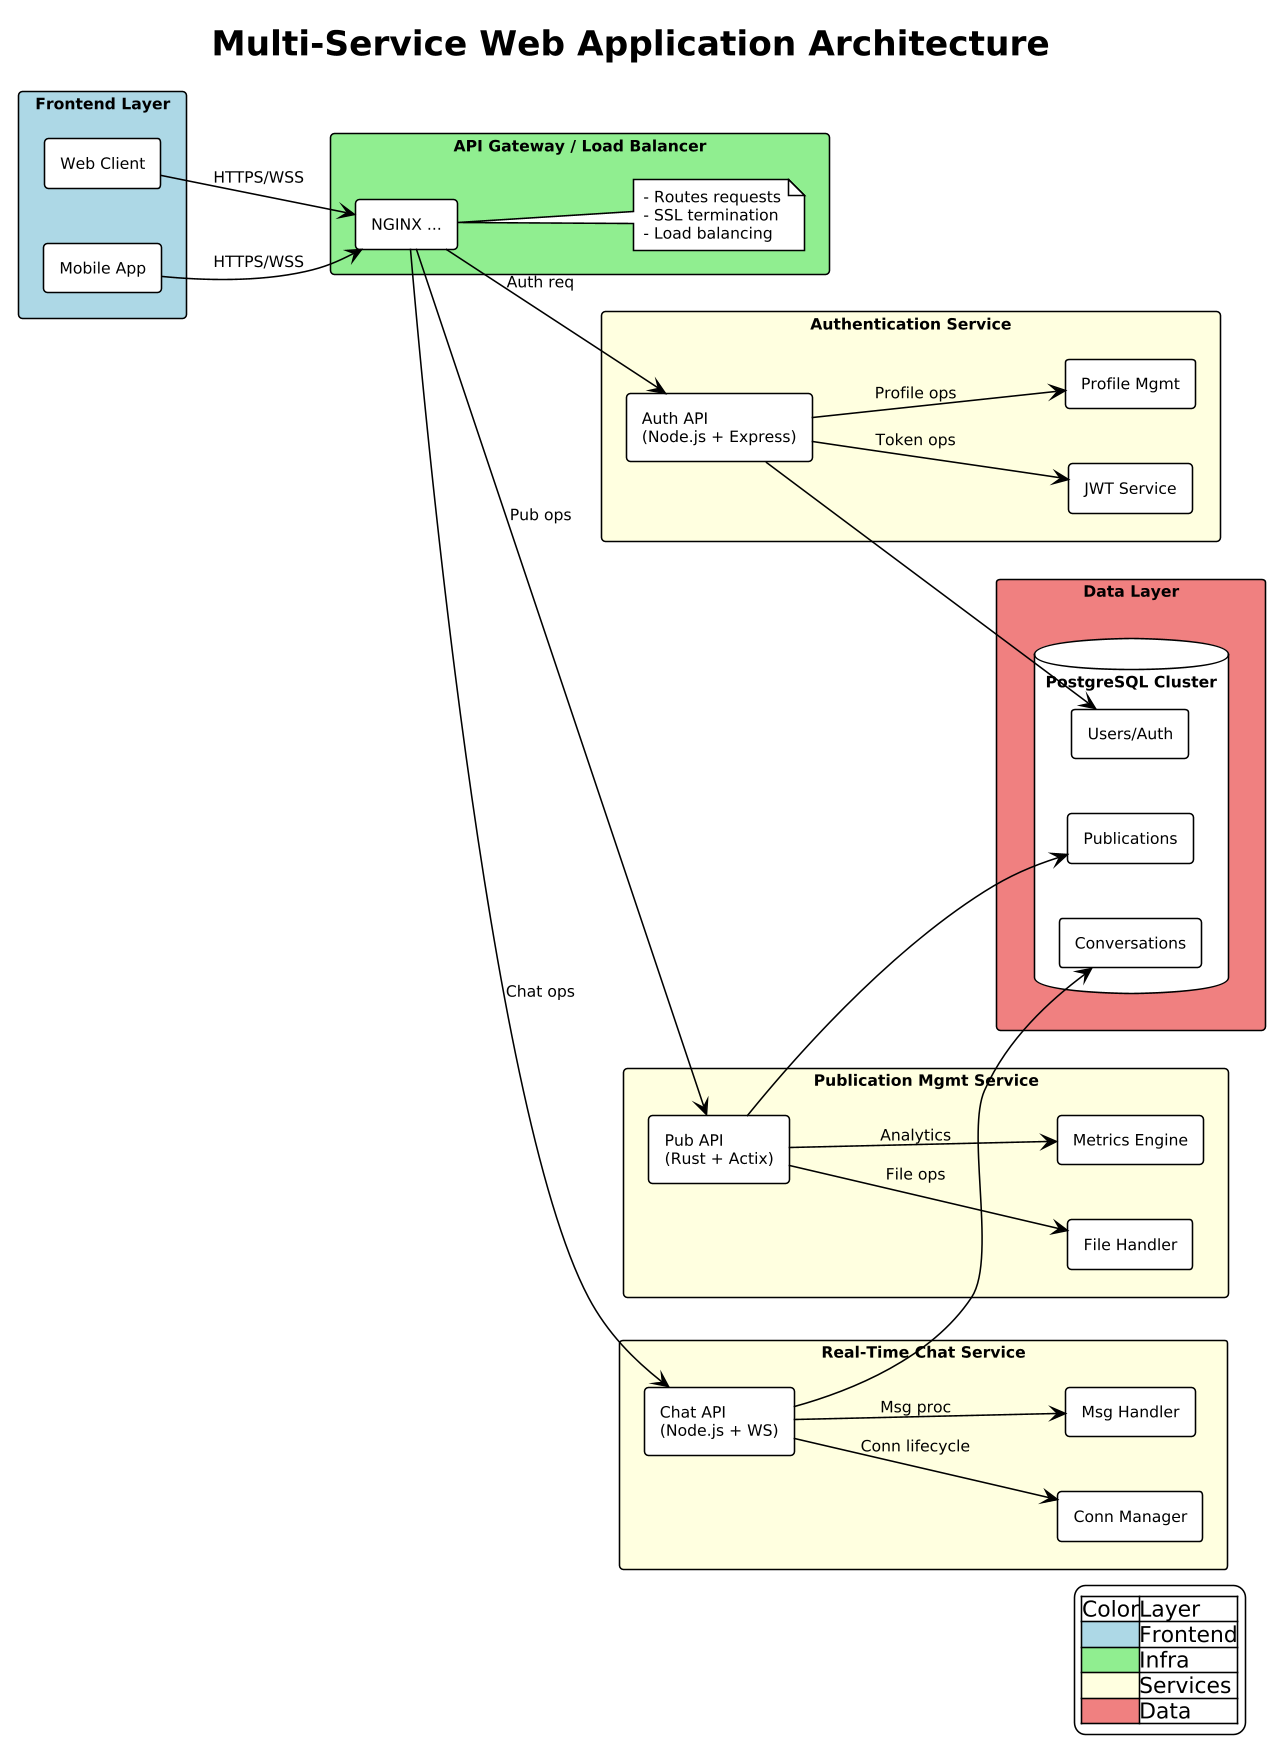
\includegraphics[width=1.0\textwidth]{diagrams/diagram.png}
    \caption{Diagramme général du système}
    \label{fig:diagram-general}
\end{figure}

\FloatBarrier
\subsection{Modèle d'interaction de service}

Ce schéma détaille les séquences d’interaction entre les services. Par exemple :

\begin{enumerate}
    \item Le client se connecte via \texttt{/auth/login} (HTTP).
    \item Le service d’authentification renvoie un JWT.
    \item Le client utilise ce token pour accéder aux publications (GET \texttt{/publications}).
    \item Le chat établit une connexion WebSocket persistante.
\end{enumerate}

\begin{figure}[htbp]
    \centering
    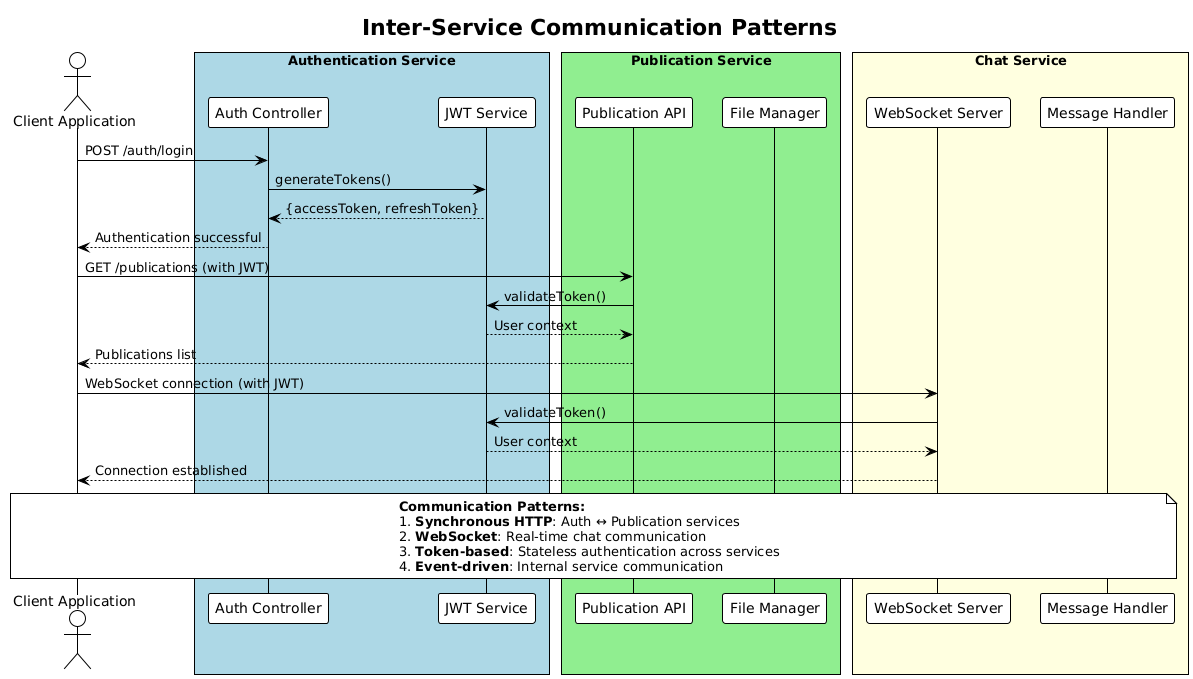
\includegraphics[width=1.1\textwidth]{diagrams/diagram1.png}
    \caption{Modèle d’Interaction de Service}
    \label{fig:diagram1}
\end{figure}

\newpage
\FloatBarrier

\section{Modèles architecturaux spécifiques aux services}

\subsection{Service d’authentification : architecture en couches}
L’architecture en couches sépare clairement les responsabilités :

\begin{itemize}
    \item La couche présentation valide les requêtes.
    \item La couche métier implémente la logique (ex. hachage de mots de passe).
    \item La couche données gère les opérations CRUD.
\end{itemize}


\begin{figure}[htbp]
    \centering
    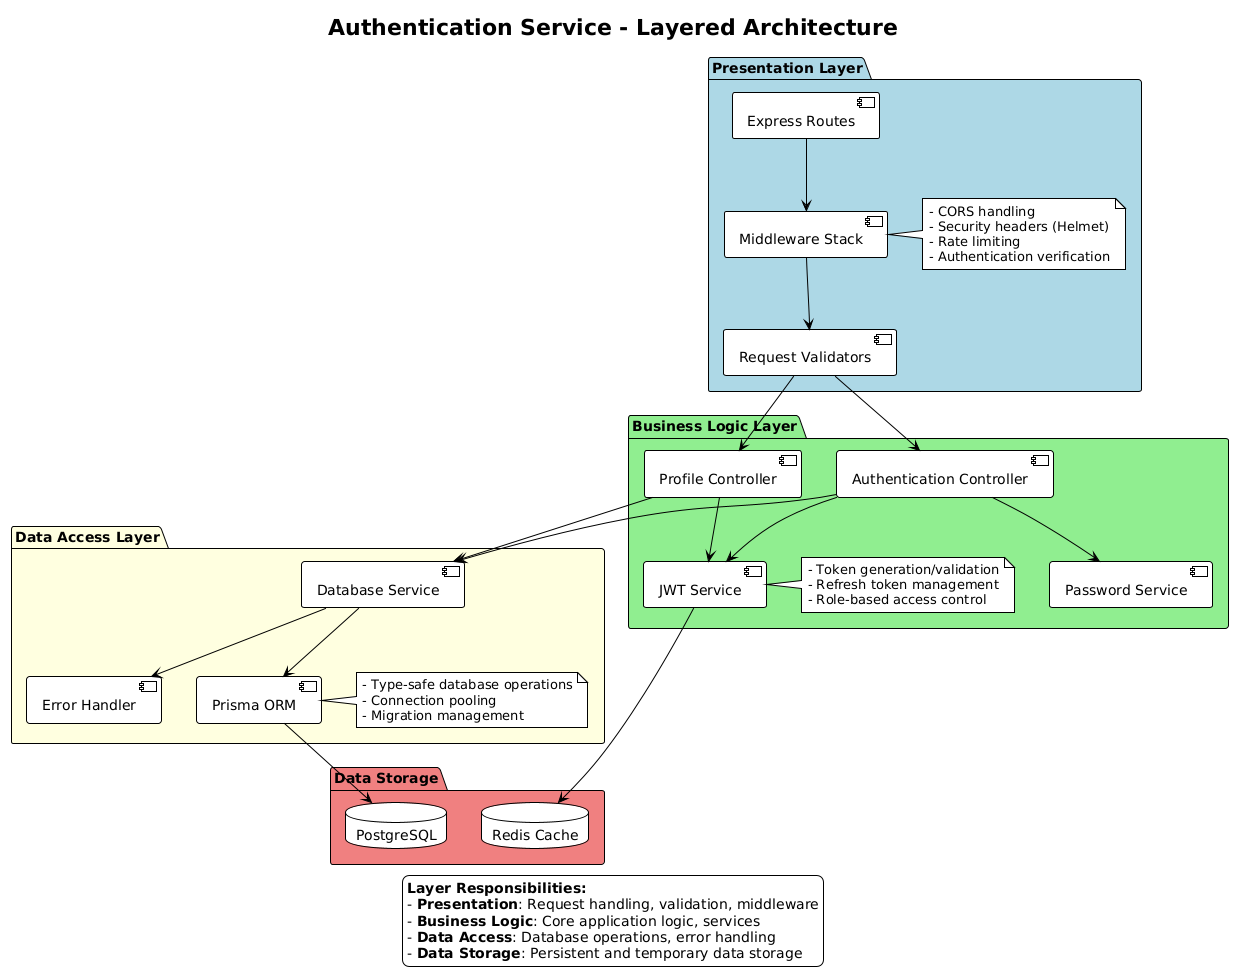
\includegraphics[width=1.1\textwidth]{diagrams/diagram2.png}
    \caption{Service d’Authentification}
    \label{fig:diagram2}
\end{figure}

\newpage
\FloatBarrier
\subsection{Service de publication : conception pilotée par le domaine}
Ce diagramme applique les principes du Domain-Driven Design (DDD) :

\begin{itemize}
    \item Les agrégats (ex. Publication) délimitent les frontières de cohérence.
    \item Les entités (ex. Conference) ont une identité unique.
    \item Les services (ex. FileService) gèrent les opérations transverses.
\end{itemize}

\begin{figure}[htbp]
    \centering
    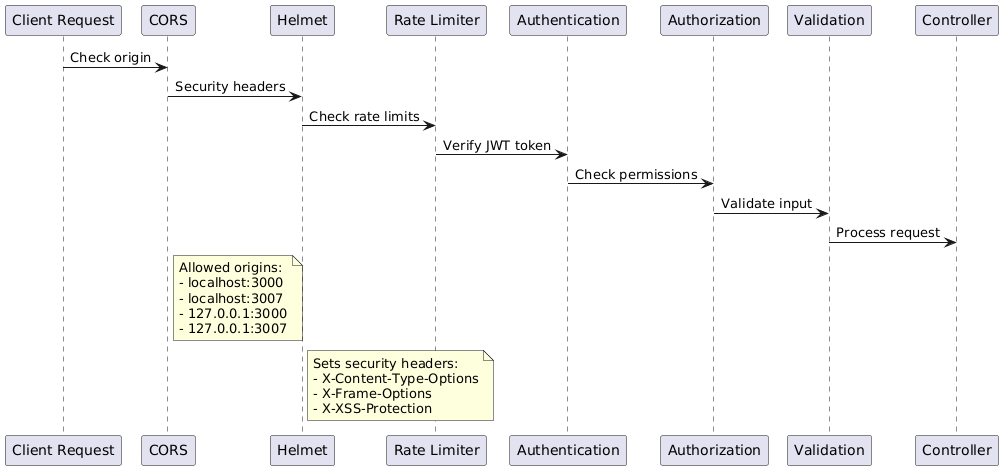
\includegraphics[width=1.1\textwidth]{diagrams/diagram3.png}
    \caption{Service de Publications }
    \label{fig:diagram3}
\end{figure}

\FloatBarrier
\subsection{Service de chat : architecture orientée événements }

Le diagramme du service de chat illustre une architecture orientée événements conçue pour gérer les interactions entre utilisateurs dans un environnement de chat en temps réel. Cette architecture est pensée pour être évolutive, modulaire, et capable de supporter un grand nombre de connexions simultanées. Elle s’appuie sur l’utilisation de WebSockets pour assurer une communication bidirectionnelle et instantanée ainsi que sur un système d’événements pour coordonner les différents composants du service.

\paragraph{Composants principaux}

\begin{itemize}
  \item \textbf{Utilisateurs (User A, User B)} \\
  \item \textbf{WebSockets (WebSocket A, WebSocket B)} \\
  Interfaces de communication en temps réel entre les utilisateurs et le serveur.

  \item \textbf{Gestionnaire de connexions (Connection Manager)} \\
  Composant chargé de gérer les connexions WebSocket, en enregistrant les connexions et déconnexions des utilisateurs, et en diffusant les mises à jour concernant la présence des utilisateurs.

  \item \textbf{Gestionnaire de messages (Message Handler)} \\
  Responsable de la réception, du traitement et de la diffusion des messages entre les participants au chat.

  \item \textbf{Bus d’événements (Event Bus)} \\
  Système de messagerie interne facilitant la communication entre les différents composants du service en transmettant les événements générés.

  \item \textbf{Base de données (Database)} \\
  Stockage persistant des messages et des informations de connexion, permettant la récupération, l’archivage et la gestion durable des données.
\end{itemize}

\begin{figure}[htbp]

    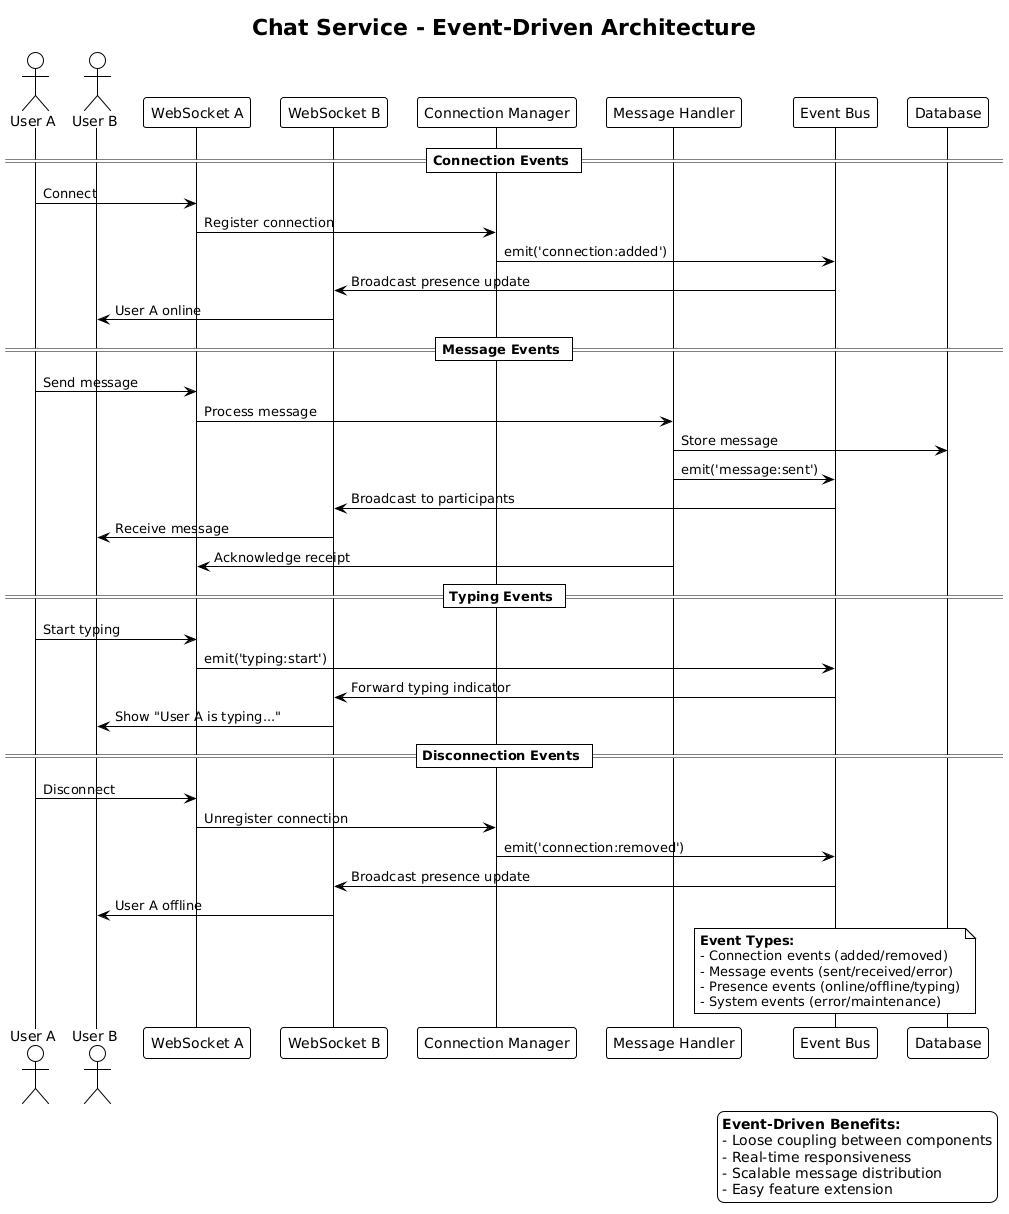
\includegraphics[width=0.93\textwidth]{diagrams/diagram4.png}
    \caption{Service de Chat}
    \label{fig:diagram4}
\end{figure}


\FloatBarrier

\section{Architecture des données}

\subsection{Schéma de base de données unifié}

Ce schéma UML montre les tables PostgreSQL et leurs relations :

\begin{itemize}
    \item \texttt{users} → \texttt{publications} (relation un-à-plusieurs).
    \item \texttt{conferences} → \texttt{participants} (relation plusieurs-à-plusieurs via une table de jointure).
    \item La table \texttt{jwt\_tokens} gère les sessions actives.
\end{itemize}

\begin{figure}[htbp]
    \centering
    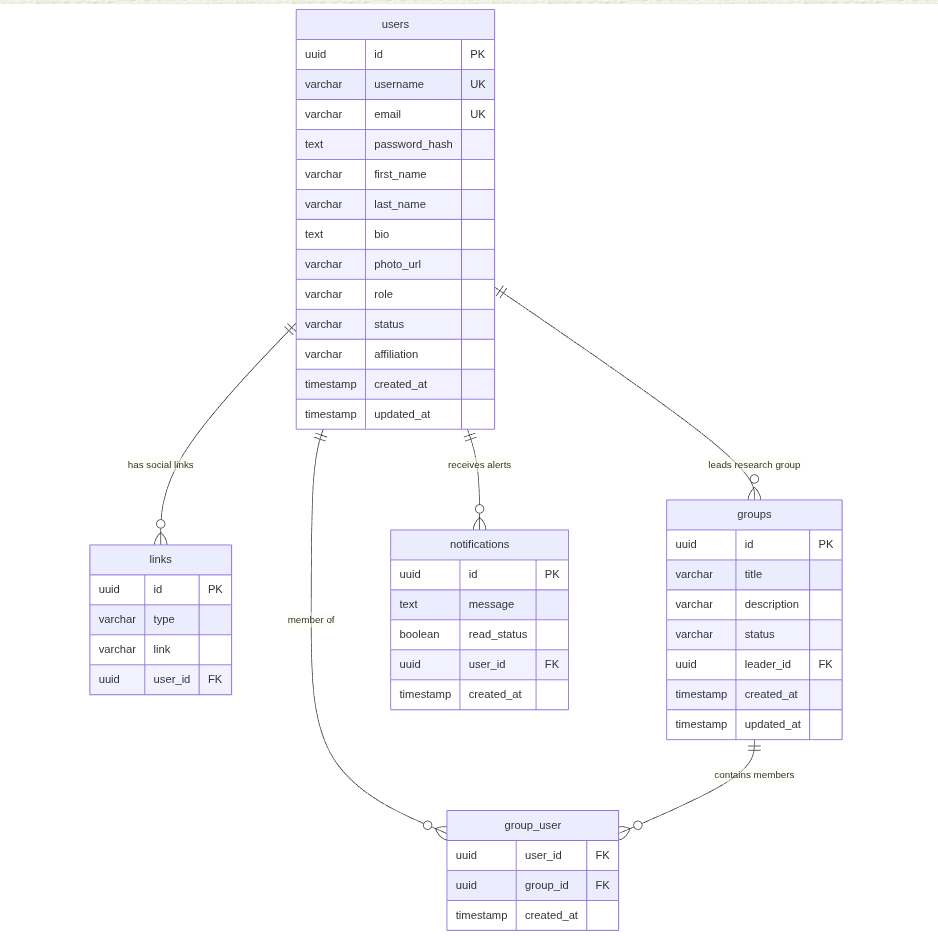
\includegraphics[width=0.8\textwidth]{diagrams/diagram5.png}
    \caption{Schéma de Base de Données}
    \label{fig:diagram5}
\end{figure}


\FloatBarrier
\newpage
\section{Architecture de sécurité}

\subsection{Modèle de sécurité multi-couches}

\subsection*{Sécurité Frontend}
\begin{itemize}
  \item \textbf{Application de HTTPS} : Assure que les communications entre le client et le serveur se font via HTTPS, chiffrant les données en transit et protégeant contre l'interception.
  \item \textbf{Politique de sécurité des contenus (Content Security Policy)} : Stratégie réduisant les vulnérabilités aux attaques par injection de scripts en spécifiant les sources valides pour le chargement des ressources.
  \item \textbf{Protection contre les attaques XSS} : Prévient les attaques Cross-Site Scripting en neutralisant les scripts malveillants exécutés dans le contexte d'un autre site.
  \item \textbf{Jetons CSRF} : Utilisés pour prévenir les attaques Cross-Site Request Forgery en s'assurant que les requêtes proviennent de la source attendue.
\end{itemize}

\subsection*{Sécurité Réseau}
\begin{itemize}
  \item \textbf{Équilibreur de charge (Load Balancer)} : Répartit le trafic entre plusieurs serveurs pour améliorer disponibilité et résilience.
  \item \textbf{Protection contre les attaques DDoS} : Détecte et bloque le trafic malveillant visant à saturer le système.
  \item \textbf{Limitation du débit (Rate Limiting)} : Restreint le nombre de requêtes par utilisateur pour prévenir abus et attaques.
  \item \textbf{Liste blanche d'IP (IP Whitelisting)} : Autorise uniquement les connexions depuis des adresses IP spécifiques.
\end{itemize}

\subsection*{Sécurité d'Authentification}
\begin{itemize}
  \item \textbf{Validation des jetons JWT} : Vérification de la validité des JSON Web Tokens.
  \item \textbf{Rotation des jetons de rafraîchissement} : Renouvellement sécurisé des jetons d'authentification.
\end{itemize}

\subsection*{Sécurité d'Autorisation}
\begin{itemize}
  \item \textbf{Contrôle d'accès basé sur les rôles (RBAC)} : Attribution des permissions selon les rôles utilisateurs.
  \item \textbf{Autorisations des ressources} : Contrôle précis des actions sur les ressources.
  \item \textbf{Protection des API} : Mesures pour sécuriser les API contre accès non autorisés.
  \item \textbf{Filtrage des données} : Prévention des injections SQL et autres attaques liées aux données.
\end{itemize}

\subsection*{Sécurité des Données}
\begin{itemize}

  \item \textbf{Hachage des mots de passe} : Stockage sécurisé des mots de passe sous forme de hash.
  \item \textbf{Validation des fichiers} : Vérification des fichiers uploadés pour éliminer les codes malveillants.
  \item \textbf{Nettoyage des entrées (Input Sanitization)} : Protection contre XSS, injections SQL, et autres vulnérabilités.
\end{itemize}

Ces éléments travaillent ensemble pour créer une architecture de sécurité robuste, couvrant les différents aspects de la protection des données et systèmes.


\begin{figure}[htbp]
    \centering
    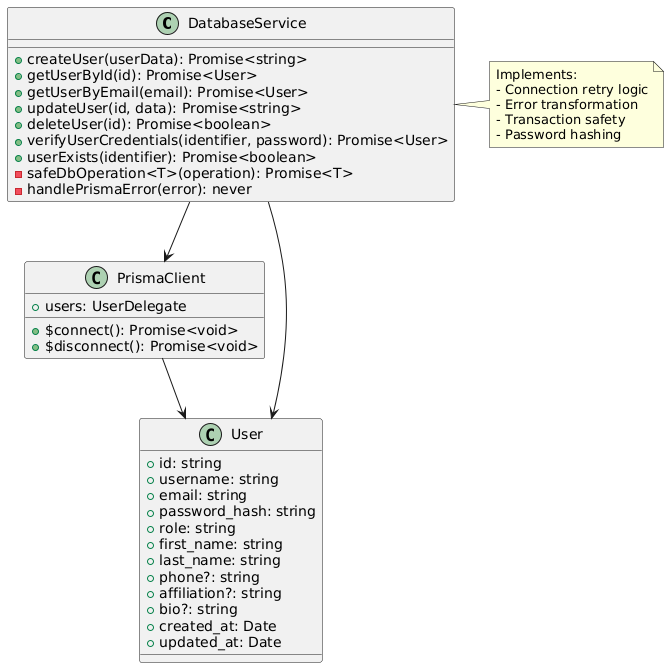
\includegraphics[width=1.1\textwidth]{diagrams/diagram6.png}
    \caption{Modèle de Sécurité Multi-Couches}
    \label{fig:diagram6}
\end{figure}



\newpage

\chapter{Mise en œuvre du site web}

\section{Gestion du code source et collaboration : GitHub}

Le choix de GitHub comme plateforme d’hébergement du code source et de collaboration a grandement contribué à industrialiser notre processus de développement, en alignant nos pratiques avec les standards professionnels actuels.

\subsection{Fonctionnalités stratégiques utilisées}

\begin{itemize}
    \item \textbf{Gestion des versions :} Chaque modification est tracée via des commits, assurant une traçabilité complète des évolutions du projet.
    \item \textbf{Travail collaboratif :} L’utilisation de branches dédiées et de pull requests permet à chaque développeur de travailler indépendamment tout en maintenant la stabilité de la branche principale.
    \item \textbf{Automatisation des validations :} L’intégration avec des outils externes permet l’exécution automatique de tests et de compilations avant toute fusion, garantissant ainsi la qualité du code.
\end{itemize}

\FloatBarrier
\begin{figure}[htbp]
    \centering
    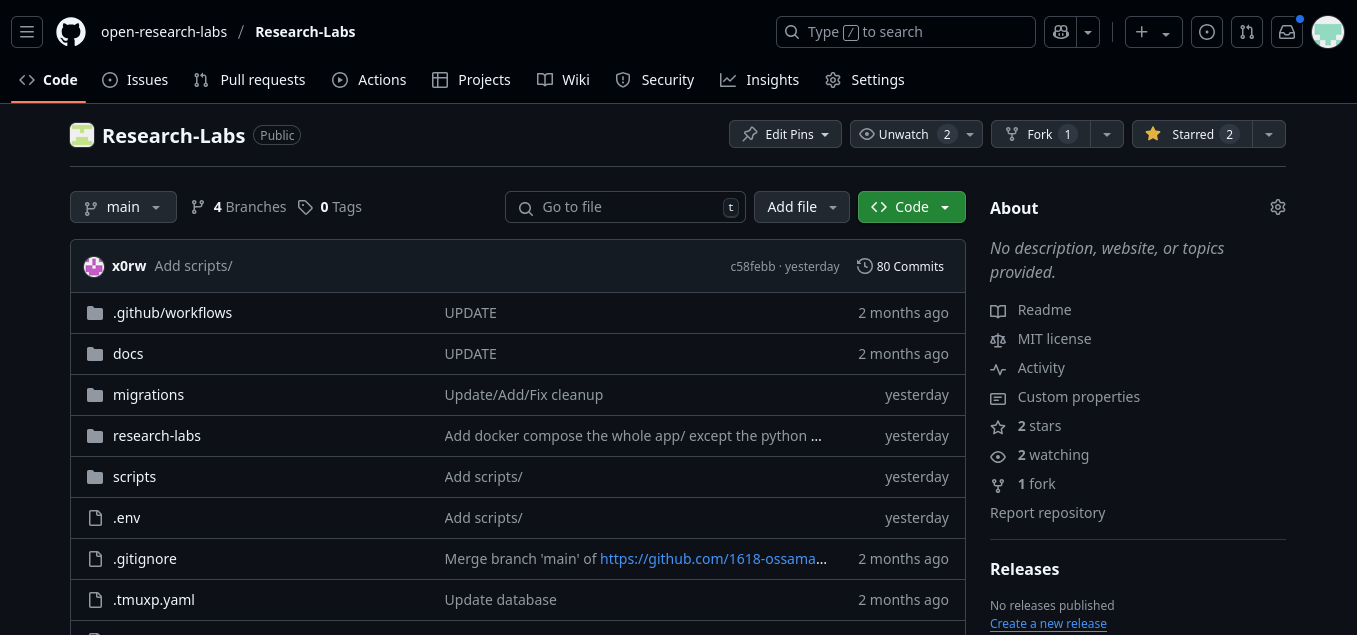
\includegraphics[width=1.0\textwidth]{diagrams/ss_02.png}
    \caption{GitHub}
    \label{fig:diagram5}
\end{figure}

\subsection{Organisation du dépôt et gestion des branches}

\begin{figure}[htbp]
    \centering
    \begin{minipage}[t]{0.3\textwidth}
        \vspace{0pt} 
        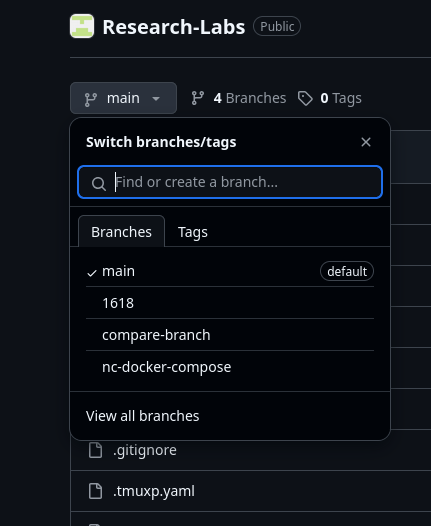
\includegraphics[width=\textwidth]{diagrams/ss_04.png}
        \caption{Branches Git}
        \label{fig:diagram5}
    \end{minipage}
    \hfill
    \begin{minipage}[t]{0.65\textwidth}
        \vspace{80pt} 
        \noindent La branche \texttt{main} conserve la version stable du projet. Pour chaque nouvelle fonctionnalité ou correction, une branche spécifique est créée. Cette organisation minimise les conflits et favorise un développement parallèle efficace.
    \end{minipage}
\end{figure}



\subsection{Demandes de fusion et revue de code}

Les pull requests assurent une revue rigoureuse du code par les membres de l’équipe, permettant la détection précoce d’erreurs, l’amélioration de la qualité du code, ainsi que le partage des connaissances.

\subsection{Suivi des tâches avec GitHub Issues}

GitHub Issues a été employé pour documenter et prioriser les tâches. Chaque problème ou nouvelle fonctionnalité fait l’objet d’une issue, facilitant la planification et le suivi de l’avancement.

\subsection{Impact global de GitHub}

Cette méthodologie a permis de centraliser le développement, faciliter le travail asynchrone, maintenir un historique détaillé des modifications, et renforcer la rigueur grâce aux revues systématiques.

\section{Tests des API : Postman}

Postman a été l’outil principal pour tester, documenter et valider les API RESTful développées. Ses fonctionnalités clés incluent :

\begin{itemize}
    \item \textbf{Environnements configurables} pour gérer les différentes phases (développement, production).
    \item \textbf{Collections organisées} permettant de regrouper les endpoints et de faciliter leur réutilisation.
    \item \textbf{Tests automatisés} écrits en JavaScript, garantissant la conformité des réponses (statut, format, performance).
    \item \textbf{Documentation dynamique} générée automatiquement pour faciliter l’intégration frontend/backend.
\end{itemize}

\FloatBarrier
\begin{figure}[htbp]
    \centering
    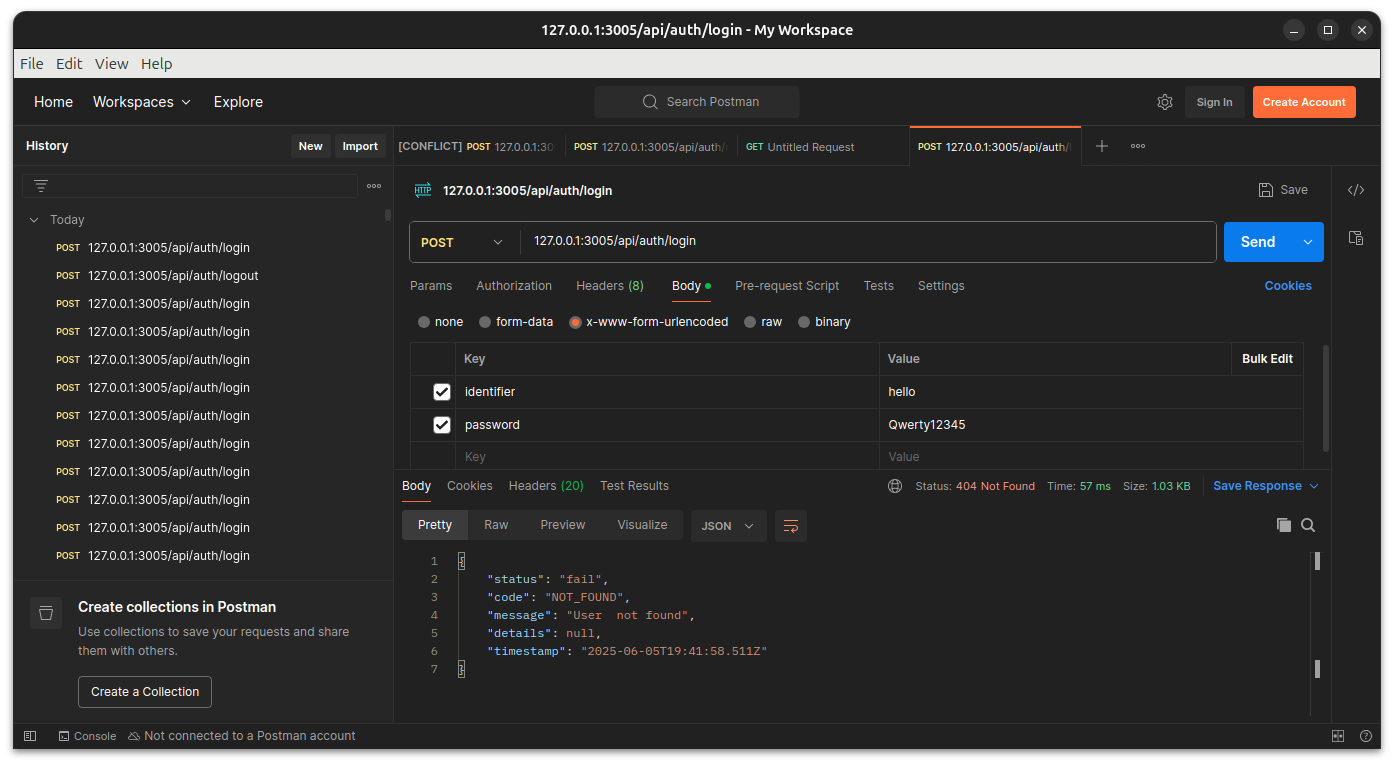
\includegraphics[width=1.0\textwidth]{diagrams/ss_05.png}
    \caption{Tests d'API}
    \label{fig:diagram5}
\end{figure}

\section{Tests des WebSockets : wscat}

Pour valider les fonctionnalités temps réel telles que les notifications ou le chat, l’outil en ligne de commande \texttt{wscat} a été utilisé :

\begin{itemize}
    \item Connexion directe aux serveurs WebSocket pour envoyer et recevoir des messages en temps réel.
    \item Tests de stabilité et de latence, permettant un débogage efficace.
    \item Facilité d’intégration dans des scripts automatisés grâce à sa compatibilité shell.
\end{itemize}

\FloatBarrier
\begin{figure}[htbp]
    \centering
    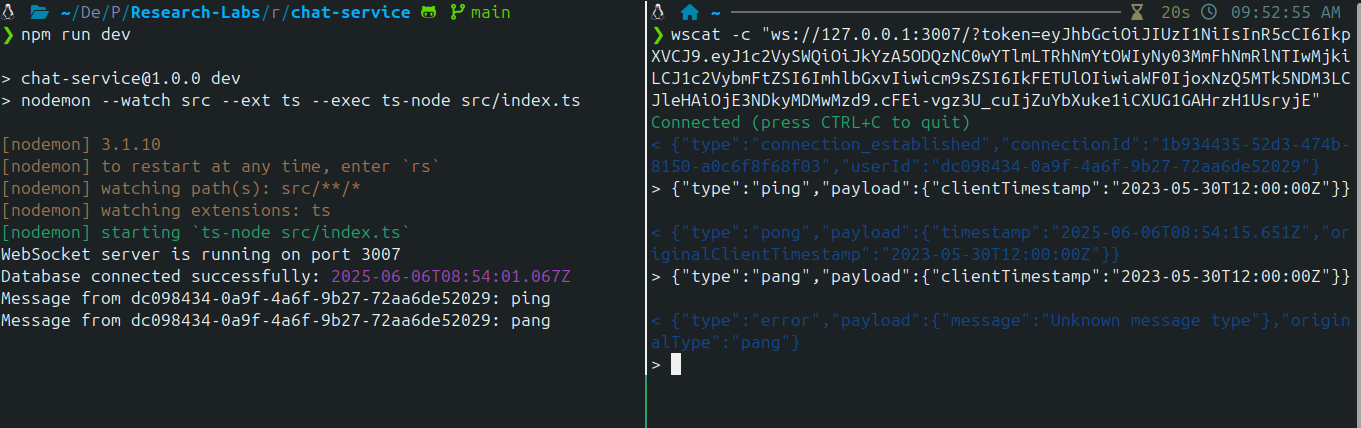
\includegraphics[width=1.0\textwidth]{diagrams/ss_08.png}
    \caption{Test du serveur chat par wscat}
    \label{fig:diagram5}
\end{figure}

une session de terminal où un serveur de chat est en cours d'exécution et communique avec un client via WebSocket. Le serveur écoute sur le port 3007 et reçoit des messages de type "ping" du client, auxquels il répond par des messages de type "pong". Cependant, le client envoie également un message de type inconnu, qui est traité par le serveur comme une erreur, illustrant comment le serveur gère les types de messages attendus et les erreurs.

\section{Gestion et interrogation des bases de données : DBeaver}

DBeaver a permis une gestion centralisée des bases de données du projet, notamment PostgreSQL, grâce à :

\begin{itemize}
    \item Un éditeur SQL puissant avec coloration syntaxique et auto-complétion.
    \item Une visualisation claire des schémas, tables, relations et index.
    \item Des fonctionnalités d’import/export pour manipuler facilement les données.
    \item La gestion sécurisée des connexions (SSH, SSL) pour protéger l’accès aux données.
\end{itemize}

\section{Conteneurisation et orchestration : Docker}

Docker a été un pilier de notre mise en œuvre, assurant la cohérence des environnements de développement et de tests.

\subsection{Mise en œuvre technique}

\begin{itemize}
    \item Utilisation de \texttt{Dockerfiles} pour définir des images reproductibles des services backend, frontend et base de données.
    \item Orchestration avec \texttt{Docker Compose} pour gérer le lancement simultané et les dépendances entre conteneurs.
    \item Volumes persistants configurés pour assurer la durabilité des données malgré la recréation des conteneurs.
\end{itemize}

\subsection{Bénéfices}

\begin{itemize}
    \item Isolation stricte des environnements pour éviter les conflits de dépendances.
    \item Portabilité permettant une exécution identique en local, en staging et en production.
    \item Préparation facilitée à la scalabilité et à l’intégration future avec Kubernetes.
    \item Intégration possible avec GitHub Actions pour automatiser les builds et tests continus.
\end{itemize}

\section{Synthèse}

Cette phase de mise en œuvre a permis d'établir une base solide pour le développement du site web, en s'appuyant sur des outils et méthodes professionnels garantissant qualité, traçabilité et collaboration efficace. Bien que le déploiement en production ne soit pas encore réalisé, toutes les préparations nécessaires ont été intégrées dès cette étape afin de faciliter cette future étape.

\section{Méthodologie de Développement}
\subsubsection{Approche Agile Adoptée}
Le projet a suivi une méthodologie \textbf{Agile} adaptée aux contraintes académiques et à la taille réduite de l'équipe. Cette approche a été structurée en sprints courts de deux semaines, avec une répartition claire des responsabilités techniques.

\paragraph{Principes Appliqués :}
\begin{itemize}
    \item \textbf{Développement itératif} : livraisons fonctionnelles toutes les deux semaines avec démonstrations à l'encadrant
    \item \textbf{Collaboration intensive} : réunions de synchronisation régulières pour coordonner les intégrations entre services
    \item \textbf{Répartition par microservice} : chaque membre était responsable d’un microservice spécifique (authentification, publications, IA, chat), garantissant autonomie et spécialisation
    \item \textbf{Mises à jour continues} : chaque service était maintenu et amélioré indépendamment, avec intégration progressive via Docker Compose
    \item \textbf{Priorité au logiciel fonctionnel} : chaque sprint visait un livrable testable plutôt qu'une documentation exhaustive
\end{itemize}


\paragraph{Organisation des sprints :}
\begin{itemize}
    \item \textbf{Sprint 1} : Architecture, Docker, auth Node.js
    \item \textbf{Sprint 2} : API Rust pour publications, téléversement
    \item \textbf{Sprint 3} : Frontend Next.js, responsive design
    \item \textbf{Sprint 4} : Chat WebSocket, intégration IA, tests
\end{itemize}

\subsubsection{Comparaison Agile vs Waterfall}
\begin{center}
\begin{tabular}{|l|l|l|}
\hline
\textbf{Critère} & \textbf{Agile (choisi)} & \textbf{Waterfall (rejeté)} \\
\hline
Flexibilité & Adaptable en cours de route & Coûteux à modifier \\
\hline
Retours & Continus & Tardifs \\
\hline
Livraisons & Incrémentales & Un bloc final \\
\hline
Documentation & Juste suffisante & Exhaustive dès le début \\
\hline
\end{tabular}
\end{center}


\subsection{Captures d'écran de l'application}

Cette section présente les différentes interfaces de l'application développée, illustrant les fonctionnalités principales à travers des captures d'écran détaillées. Chaque interface a été conçue pour offrir une expérience utilisateur optimale tout en respectant les principes d'ergonomie et d'accessibilité.

\subsubsection{Interface de connexion}

\begin{figure}[H]
    \centering
    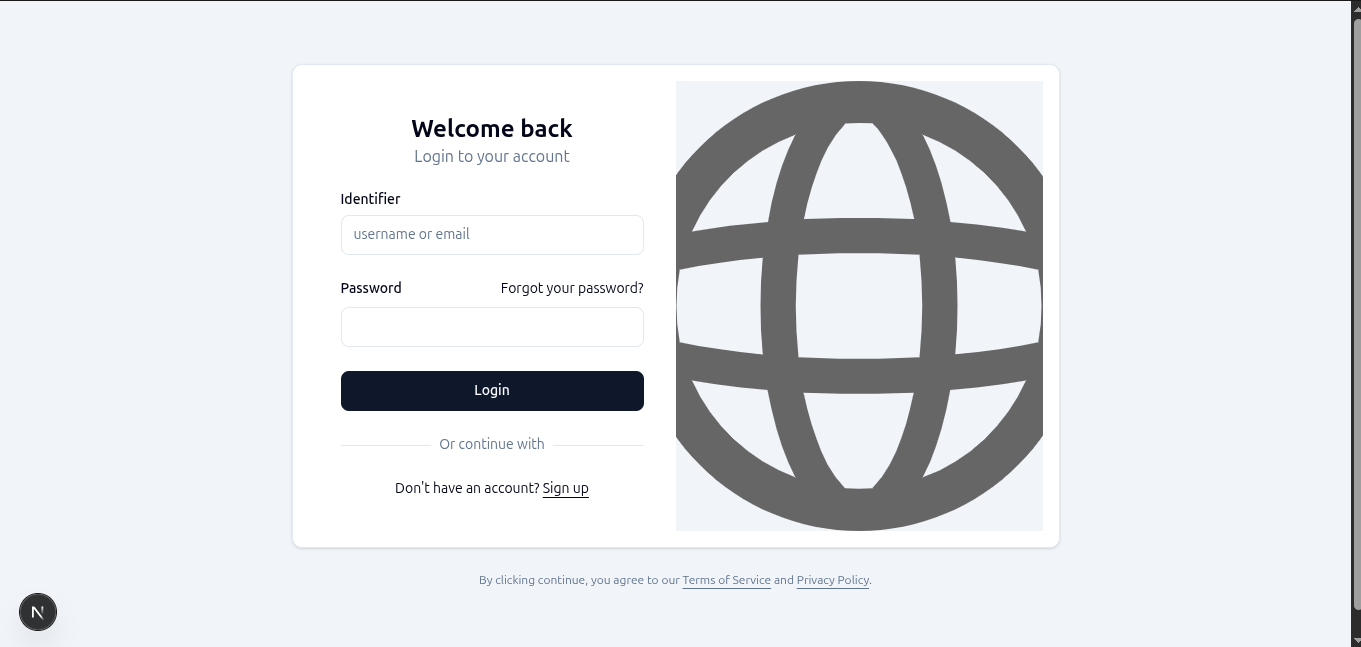
\includegraphics[width=0.8\textwidth]{diagrams/a_ss_02.png}
    \caption{Interface de connexion utilisateur}
    \label{fig:login}
\end{figure}

L'interface de connexion présente un design épuré et professionnel, caractérisé par :
\begin{itemize}
    \item \textbf{Validation en temps réel} : Les champs de saisie affichent instantanément les erreurs de format ou les champs manquants
    \item \textbf{Messages d'erreur contextuels} : Affichage de messages clairs en cas d'échec d'authentification
    \item \textbf{Design responsive} : Interface adaptée aux différentes tailles d'écran
    \item \textbf{Sécurité visuelle} : Masquage automatique du mot de passe avec option d'affichage temporaire
\end{itemize}

\subsubsection{Tableau de bord principal}

\begin{figure}[H]
    \centering
    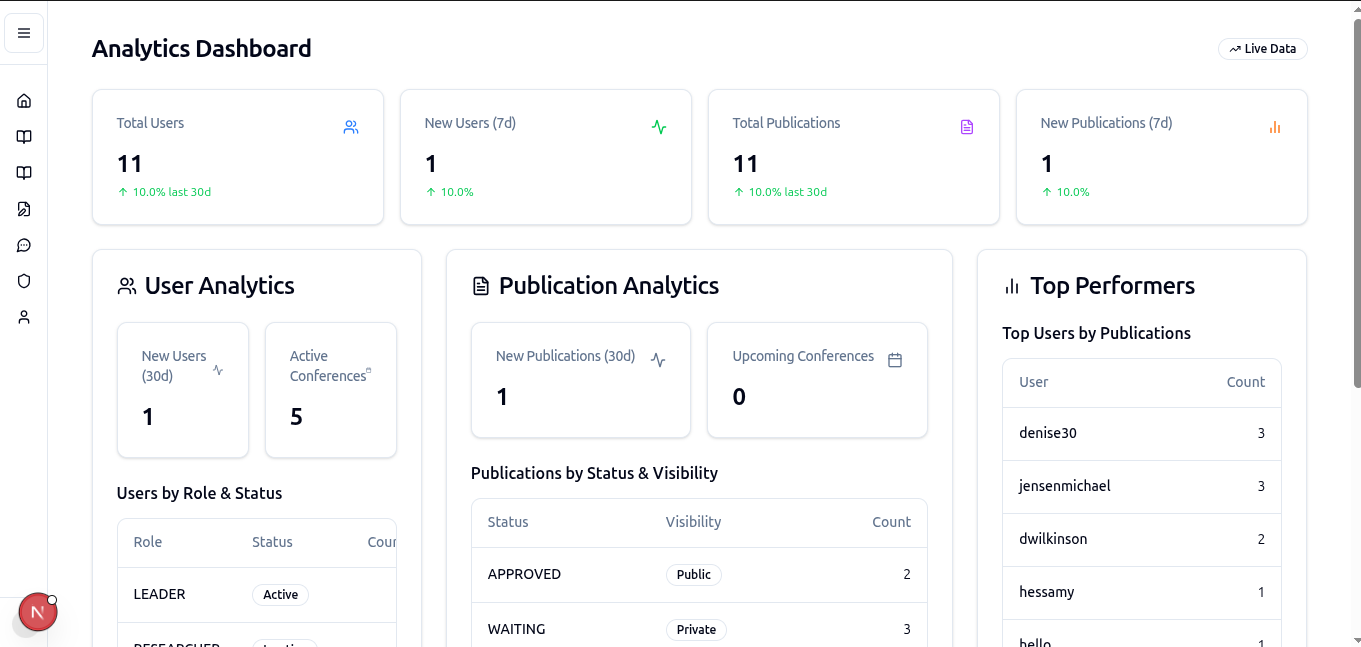
\includegraphics[width=0.9\textwidth]{diagrams/a_ss_08.png}
    \caption{Tableau de bord principal avec métriques et aperçu}
    \label{fig:dashboard}
\end{figure}

Le tableau de bord offre une vue d'ensemble complète des activités du laboratoire :
\begin{itemize}
    \item \textbf{Métriques en temps réel} : Statistiques sur les publications, conférences et membres actifs
    \item \textbf{Publications récentes} : Aperçu des dernières publications ajoutées avec leurs statuts
    \item \textbf{Notifications} : Système d'alertes pour les échéances importantes et les nouvelles activités
    \item \textbf{Navigation intuitive} : Menu latéral avec accès rapide à toutes les fonctionnalités
\end{itemize}

\subsubsection{Module de gestion des publications}

\begin{figure}[H]
    \centering
    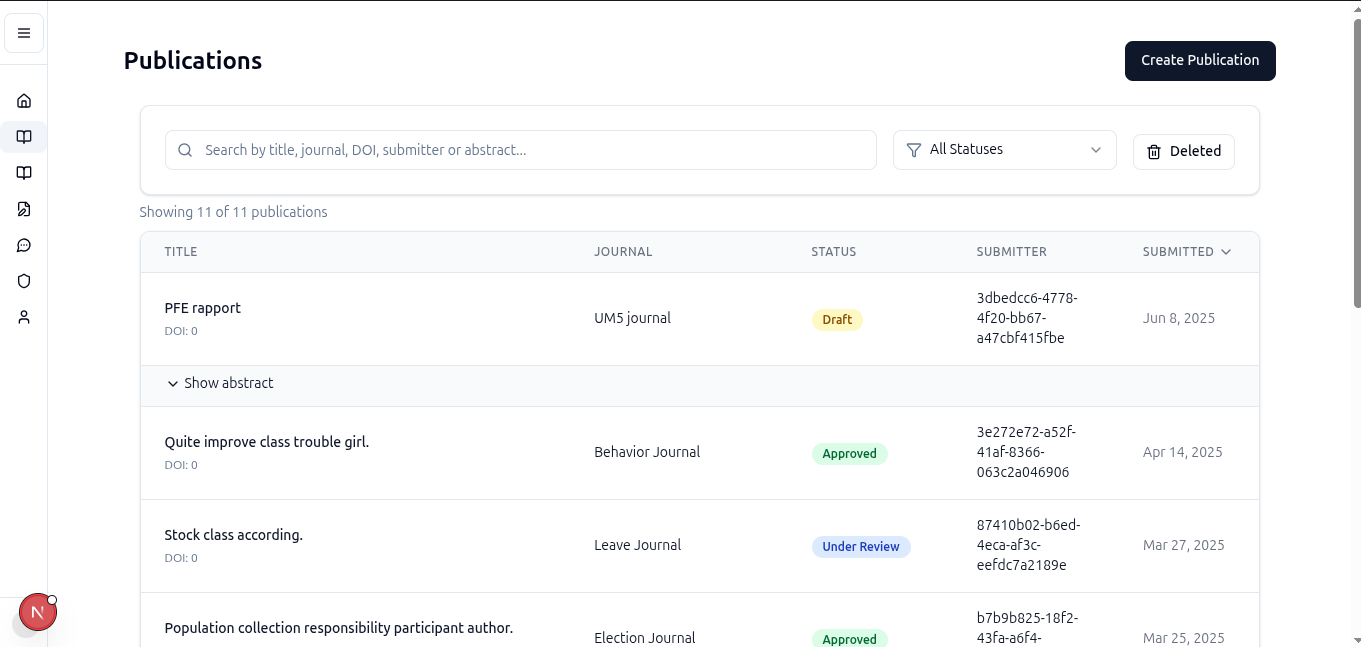
\includegraphics[width=0.9\textwidth]{diagrams/a_ss_12.png}
    \caption{Interface de gestion des publications avec filtres et pagination}
    \label{fig:publications}
\end{figure}

\begin{figure}[H]
    \centering
    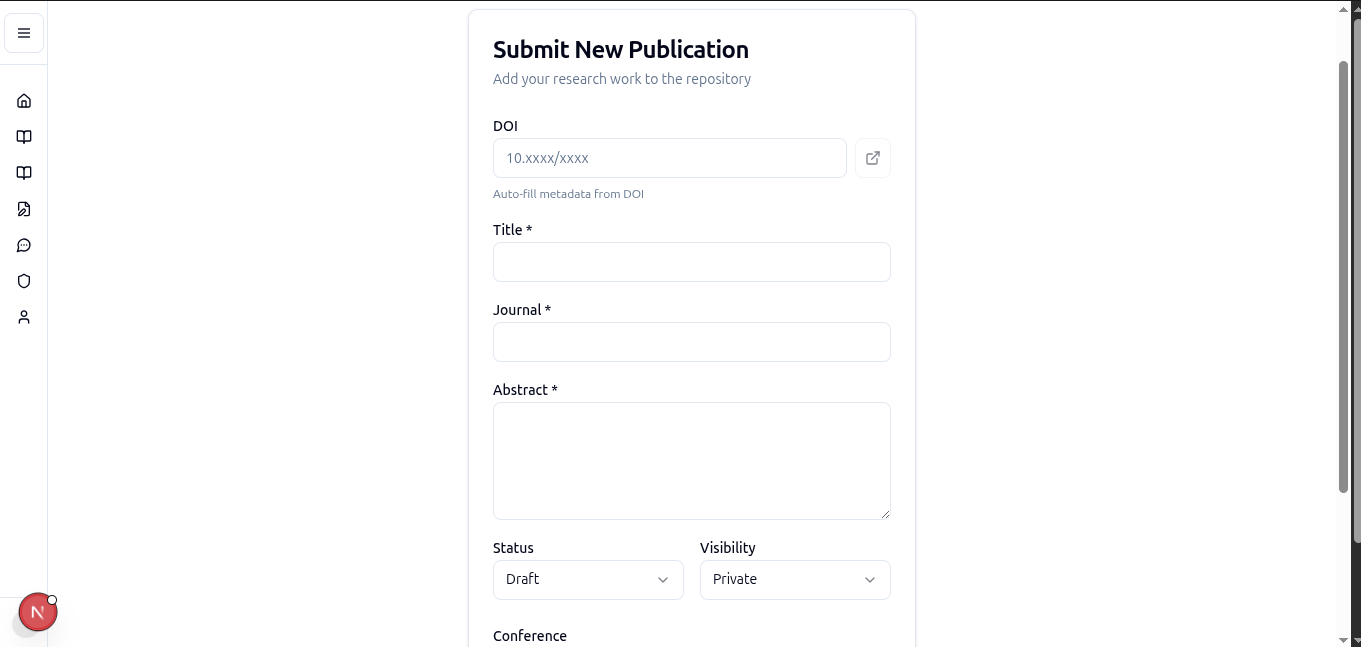
\includegraphics[width=0.8\textwidth]{diagrams/a_ss_11.png}
    \caption{Formulaire d'ajout d'une nouvelle publication}
    \label{fig:add_publication}
\end{figure}

Le module publications comprend des fonctionnalités avancées :
\begin{itemize}
    \item \textbf{Filtres dynamiques} : Recherche par auteur, date, type de publication, et mots-clés
    \item \textbf{Pagination intelligente} : Navigation fluide à travers de grandes collections de données
    \item \textbf{Formulaire d'ajout complet} : Saisie structurée avec validation des champs obligatoires
    \item \textbf{Upload de fichiers PDF} : Glisser-déposer avec prévisualisation et validation du format
    \item \textbf{Métadonnées enrichies} : Gestion des co-auteurs, affiliations, et classifications
\end{itemize}

\subsubsection{Intégration de l'intelligence artificielle}

\begin{figure}[H]
    \centering
    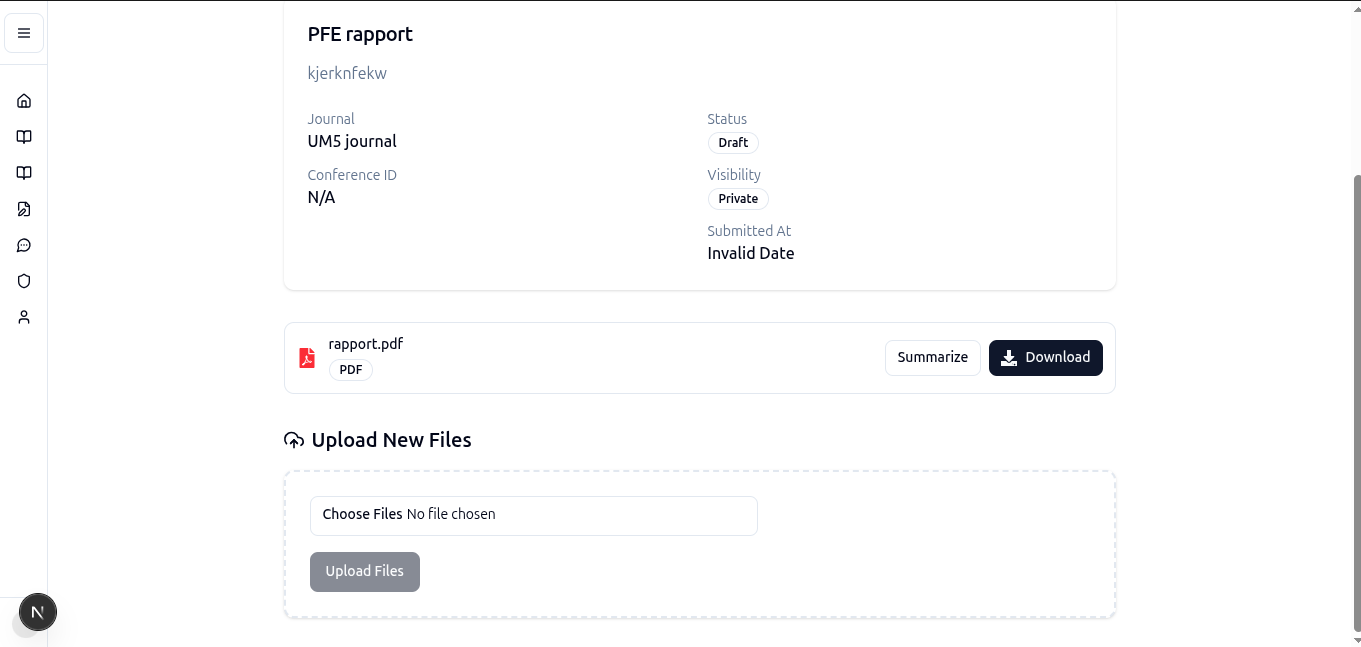
\includegraphics[width=0.9\textwidth]{diagrams/a_ss_13.png}
    \caption{Génération automatique de résumés par intelligence artificielle}
    \label{fig:ai_summary}
\end{figure}

L'interface d'IA démontre les capacités avancées du système :
\begin{itemize}
    \item \textbf{Résumés automatiques} : Génération de synthèses à partir du contenu des publications PDF
    \item \textbf{Analyse sémantique} : Extraction des concepts clés et des contributions principales
    \item \textbf{Interface de révision} : Possibilité d'éditer et valider les résumés générés
    \item \textbf{Indicateurs de qualité} : Score de confiance et métriques sur la précision du résumé
\end{itemize}

\subsubsection{Système de messagerie instantanée}

\begin{figure}[H]
    \centering
    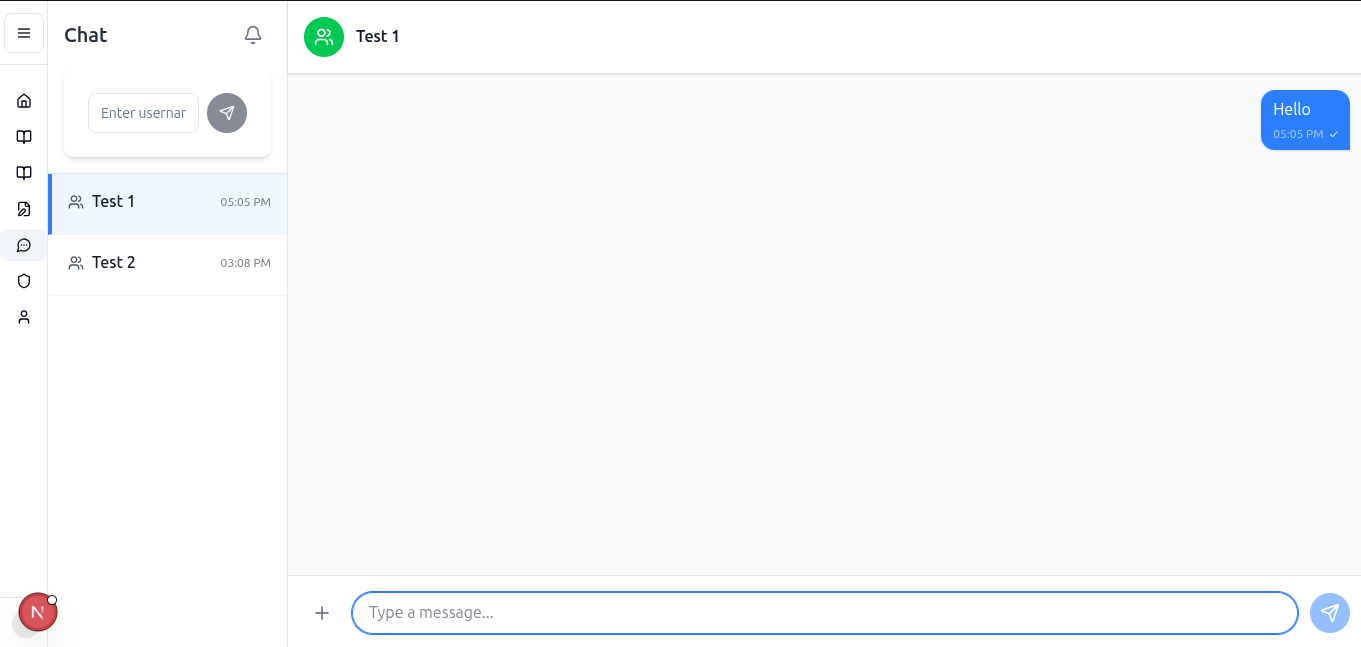
\includegraphics[width=0.9\textwidth]{diagrams/a_ss_06.png}
    \caption{Interface de chat avec liste des utilisateurs et groups}
    \label{fig:chat}
\end{figure}

Le système de chat offre une communication fluide :
\begin{itemize}
    \item \textbf{Groupes de messagerie} : Création de salons de discussion pour les équipes ou projets
    \item \textbf{Messages instantanés} : Communication bidirectionnelle via WebSockets
    \item \textbf{Historique persistant} : Conservation et recherche dans l'historique des conversations
    \item \textbf{Notifications push} : Alertes pour les nouveaux messages et mentions
    \item \textbf{Interface adaptative} : Design optimisé pour les conversations longues
\end{itemize}

\subsubsection{Analyse de l'expérience utilisateur}

Les captures d'écran révèlent plusieurs aspects importants de l'interface :

\paragraph{Cohérence visuelle}
L'ensemble de l'application maintient une identité graphique homogène avec une palette de couleurs professionnelle, une typographie lisible et des éléments d'interface standardisés.

\paragraph{Ergonomie et utilisabilité}
Chaque écran respecte les principes d'ergonomie web avec des zones de contenu bien délimitées, une hiérarchie visuelle claire et des actions intuitives.

\paragraph{Feedback utilisateur}
Les interfaces intègrent des mécanismes de retour (loading states, confirmations, messages d'erreur) pour guider l'utilisateur dans ses interactions.

Cette présentation visuelle confirme que l'application répond aux exigences fonctionnelles tout en offrant une expérience utilisateur moderne et professionnelle, adaptée aux besoins spécifiques d'un laboratoire de recherche.

\newpage
\section{Conclusion Générale étendue}
Ce projet constitue une réponse concrète aux défis de gestion des laboratoires modernes. En plus de l'implémentation technique, nous avons mis l'accent sur les aspects organisationnels et les bonnes pratiques professionnelles.

\paragraph{Défis et solutions}
\begin{itemize}
    \item \textbf{Coordination microservices} : API Gateway, standards REST
    \item \textbf{Performance IA} : Redis cache + traitement async
    \item \textbf{Technologies multiples} : documentation, apprentissage continu
\end{itemize}

\paragraph{Alignement avec les objectifs secondaires}
\begin{itemize}
    \item Automatisation des tâches (upload, résumés, notifs)
    \item Centralisation des échanges (chat + tableau de bord)
    \item Sécurité (JWT, RBAC, audit)
    \item Évolutivité (Docker , Kubernetes prévu)
\end{itemize}

\paragraph{Perspectives}
\begin{itemize}
    \item Amélioration IA (modèles GPT-4)
    \item Dashboards analytiques (D3.js)
    \item CI/CD avec GitHub Actions, monitoring Prometheus
    \item Modules futurs : gestion de projets, revue par pairs, intégration PubMed
    \item Adoption : pilote universitaire, extension, commercialisation SaaS
\end{itemize}

\paragraph{Impact}
\begin{itemize}
    \item Compétences : Rust, TS, Python, DevOps, IA
    \item Méthodes pro : Agile, TDD, doc technique, outils collaboratifs
\end{itemize}




% ... Répétez pour diagram3.png à diagram27.png ...
\newpage
\chapter*{Conclusion Générale}
\addcontentsline{toc}{chapter}{Conclusion Générale}
Ce projet s’inscrit dans une volonté d’améliorer la gestion des activités de recherche à travers une plateforme centralisée.Il pose les bases d'un écosystème digital unifié pour la recherche, conciliant technologie, ergonomie et productivité scientifique. Grâce à une architecture moderne basée sur des microservices, une base de données PostgreSQL, une interface intuitive et une sécurité renforcée, l’application répond aux besoins croissants des laboratoires universitaires. Les perspectives d’évolution incluent l’intégration d’outils analytiques avancés et l’extension vers d’autres structures de recherche.

\newpage
\bibliographystyle{plain}
\bibliography{refs}
\chapter*{Bibliographie}
\begin{thebibliography}{10}

\bibitem{richardson2018}
C.~Richardson, \textit{Microservices Patterns: With Examples in Java}. Manning Publications, 2018.

\bibitem{evans2003}
E.~Evans, \textit{Domain-Driven Design: Tackling Complexity in the Heart of Software}. Addison-Wesley Professional, 2003.

\bibitem{fowler2014}
M.~Fowler, ``Microservices,'' \textit{martinfowler.com}, Mar. 2014. [Online]. Available: \url{https://martinfowler.com/articles/microservices.html}

\bibitem{postgresql2024}
PostgreSQL Global Development Group, ``PostgreSQL Documentation,'' \textit{postgresql.org}, 2024. [Online]. Available: \url{https://www.postgresql.org/docs/}

\bibitem{mdn2024}
Mozilla Developer Network, ``WebSocket API,'' \textit{developer.mozilla.org}, 2024. [Online]. Available: \url{https://developer.mozilla.org/en-US/docs/Web/API/WebSocket}

\bibitem{docker2024}
Docker Inc., ``Docker Documentation,'' \textit{docs.docker.com}, 2024. [Online]. Available: \url{https://docs.docker.com/}

\bibitem{nextjs2024}
Next.js Team, ``Next.js Documentation,'' \textit{nextjs.org}, 2024. [Online]. Available: \url{https://nextjs.org/docs}

\bibitem{rust2024}
Rust Foundation, ``The Rust Programming Language,'' \textit{doc.rust-lang.org}, 2024. [Online]. Available: \url{https://doc.rust-lang.org/}

\bibitem{owasp2021}
OWASP Foundation, ``OWASP Top Ten Web Application Security Risks,'' \textit{owasp.org}, 2021.

\bibitem{w3c2023}
T.~Berners-Lee \textit{et al.}, ``Web Security,'' \textit{W3C}, 2023.

\bibitem{haverbeke2018}
M.~Haverbeke, \textit{Eloquent JavaScript: A Modern Introduction to Programming}, 3rd ed. No Starch Press, 2018.

\end{thebibliography}


\end{document}
